% Options for packages loaded elsewhere
\PassOptionsToPackage{unicode}{hyperref}
\PassOptionsToPackage{hyphens}{url}
\PassOptionsToPackage{dvipsnames,svgnames,x11names}{xcolor}
%
\documentclass[
  10pt,
]{article}
\usepackage{amsmath,amssymb}
\usepackage{lmodern}
\usepackage{iftex}
\ifPDFTeX
  \usepackage[T1]{fontenc}
  \usepackage[utf8]{inputenc}
  \usepackage{textcomp} % provide euro and other symbols
\else % if luatex or xetex
  \usepackage{unicode-math}
  \defaultfontfeatures{Scale=MatchLowercase}
  \defaultfontfeatures[\rmfamily]{Ligatures=TeX,Scale=1}
\fi
% Use upquote if available, for straight quotes in verbatim environments
\IfFileExists{upquote.sty}{\usepackage{upquote}}{}
\IfFileExists{microtype.sty}{% use microtype if available
  \usepackage[]{microtype}
  \UseMicrotypeSet[protrusion]{basicmath} % disable protrusion for tt fonts
}{}
\makeatletter
\@ifundefined{KOMAClassName}{% if non-KOMA class
  \IfFileExists{parskip.sty}{%
    \usepackage{parskip}
  }{% else
    \setlength{\parindent}{0pt}
    \setlength{\parskip}{6pt plus 2pt minus 1pt}}
}{% if KOMA class
  \KOMAoptions{parskip=half}}
\makeatother
\usepackage{xcolor}
\usepackage[margin=1.7cm]{geometry}
\usepackage{longtable,booktabs,array}
\usepackage{calc} % for calculating minipage widths
% Correct order of tables after \paragraph or \subparagraph
\usepackage{etoolbox}
\makeatletter
\patchcmd\longtable{\par}{\if@noskipsec\mbox{}\fi\par}{}{}
\makeatother
% Allow footnotes in longtable head/foot
\IfFileExists{footnotehyper.sty}{\usepackage{footnotehyper}}{\usepackage{footnote}}
\makesavenoteenv{longtable}
\usepackage{graphicx}
\makeatletter
\def\maxwidth{\ifdim\Gin@nat@width>\linewidth\linewidth\else\Gin@nat@width\fi}
\def\maxheight{\ifdim\Gin@nat@height>\textheight\textheight\else\Gin@nat@height\fi}
\makeatother
% Scale images if necessary, so that they will not overflow the page
% margins by default, and it is still possible to overwrite the defaults
% using explicit options in \includegraphics[width, height, ...]{}
\setkeys{Gin}{width=\maxwidth,height=\maxheight,keepaspectratio}
% Set default figure placement to htbp
\makeatletter
\def\fps@figure{htbp}
\makeatother
\setlength{\emergencystretch}{3em} % prevent overfull lines
\providecommand{\tightlist}{%
  \setlength{\itemsep}{0pt}\setlength{\parskip}{0pt}}
\setcounter{secnumdepth}{-\maxdimen} % remove section numbering
\ifLuaTeX
\usepackage[bidi=basic]{babel}
\else
\usepackage[bidi=default]{babel}
\fi
\babelprovide[main,import]{spanish}
% get rid of language-specific shorthands (see #6817):
\let\LanguageShortHands\languageshorthands
\def\languageshorthands#1{}

\usepackage{float}
\floatplacement{figure}{H}
\usepackage{iftex}
\ifPDFTeX
  \DeclareUnicodeCharacter{2192}{\ensuremath{\rightarrow}}
  \DeclareUnicodeCharacter{2248}{\ensuremath{\approx}}
  \DeclareUnicodeCharacter{2265}{\ensuremath{\geq}}
\else
  \usepackage{newunicodechar}
  \newunicodechar{→}{\ensuremath{\rightarrow}}
  \newunicodechar{≈}{\ensuremath{\approx}}
  \newunicodechar{≥}{\ensuremath{\geq}}
\fi
\ifLuaTeX
  \usepackage{selnolig}  % disable illegal ligatures
\fi
\IfFileExists{bookmark.sty}{\usepackage{bookmark}}{\usepackage{hyperref}}
\IfFileExists{xurl.sty}{\usepackage{xurl}}{} % add URL line breaks if available
\urlstyle{same} % disable monospaced font for URLs
\hypersetup{
  pdftitle={Trabajo Práctico 2 --- Trabajo 2 (eje Drama)},
  pdfauthor={Matías Adell · Agustín Giannice · Facundo Mazzola},
  pdflang={es},
  colorlinks=true,
  linkcolor={Maroon},
  filecolor={Maroon},
  citecolor={Blue},
  urlcolor={Blue},
  pdfcreator={LaTeX via pandoc}}

\title{Trabajo Práctico 2 --- Trabajo 2 (eje Drama)}
\usepackage{etoolbox}
\makeatletter
\providecommand{\subtitle}[1]{% add subtitle to \maketitle
  \apptocmd{\@title}{\par {\large #1 \par}}{}{}
}
\makeatother
\subtitle{Bases de Datos Orientadas a Grafos · UCA · 2.º cuatrimestre
2026 · Docente: José Canelón}
\author{Matías Adell · Agustín Giannice · Facundo Mazzola}
\date{Noviembre de 2026}

\begin{document}
\maketitle

\hypertarget{entorno-datos-y-muxe9todo}{%
\subsection{Entorno, datos y método}\label{entorno-datos-y-muxe9todo}}

\begin{itemize}
\tightlist
\item
  \textbf{Entorno.} Neo4j Desktop 2.2.1 con un DBMS local \textbf{Neo4j
  2026.09.0 Enterprise}, \textbf{GDS 2026.09.0} y \textbf{APOC
  2026.09.0} (heap de 4 GB, page cache de 1 GB). El notebook corre en un
  env conda en CPU (PyKEEN 1.11.1, torch 2.15 CPU).
\item
  \textbf{Carga.} El grafo se restauró desde el volcado
  \texttt{recommendations-50.dump}, sin \texttt{LOAD\ CSV}. En Desktop 2
  no existe la sección \emph{Files}: se usó \emph{Create instance} con
  el archivo del dump.
\item
  \textbf{Scripts.} Los cuatro \texttt{.cypher} (parte común y Ej. 1--3)
  son \textbf{reejecutables}: arrancan liberando lo que crean
  (\texttt{gds.graph.drop}, \texttt{gds.pipeline.drop} y
  \texttt{gds.model.drop} con \texttt{false}) y deshacen propiedades e
  índices propios. Se ejecutaron paso a paso con un \emph{runner} en
  Python (driver \texttt{neo4j}, en autocommit) que guarda cada
  resultado como evidencia.
\item
  \textbf{Indicaciones.} Semilla 42 en todo lo que la acepta,
  proyecciones UNDIRECTED y los nombres de la consigna (\texttt{califW},
  \texttt{ratingNorm}).
\item
  \textbf{Película ancla.} La película de Drama con más
  \texttt{{[}:RATED{]}} es \textbf{Forrest Gump (1994)}, con 341
  calificaciones. Se recalcula dentro de cada consulta; no está escrita
  a mano.
\end{itemize}

\hypertarget{parte-comuxfan-suxedntesis}{%
\subsection{Parte común --- síntesis}\label{parte-comuxfan-suxedntesis}}

\textbf{Panorama.} El grafo tiene \textbf{28.863 nodos y 166.261
relaciones}, que coinciden con la consigna: sí. Una \texttt{:Person}
puede ser \texttt{:Actor} y \texttt{:Director} a la vez (487 lo son),
por eso las etiquetas suman más que el total.

\begin{longtable}[]{@{}ll@{}}
\toprule()
Etiqueta & Nodos \\
\midrule()
\endhead
Person & 19.047 \\
Actor & 15.443 \\
Movie & 9.125 \\
Director & 4.091 \\
User & 671 \\
Genre & 20 \\
\bottomrule()
\end{longtable}

\begin{longtable}[]{@{}ll@{}}
\toprule()
Tipo de relación & Relaciones \\
\midrule()
\endhead
RATED & 100.004 \\
ACTED\_IN & 35.910 \\
IN\_GENRE & 20.340 \\
DIRECTED & 10.007 \\
\bottomrule()
\end{longtable}

\textbf{Las 3 películas con más calificaciones:}

\begin{longtable}[]{@{}lll@{}}
\toprule()
Película & Año & Calificaciones \\
\midrule()
\endhead
Forrest Gump & 1994 & 341 \\
Pulp Fiction & 1994 & 324 \\
Shawshank Redemption, The & 1994 & 311 \\
\bottomrule()
\end{longtable}

\textbf{Recomendación base (sin GDS) para la ancla.} Se usa el patrón
\texttt{(:Movie)\textless{}-{[}:RATED{]}-(:User)-{[}:RATED{]}-\textgreater{}(rec:Movie)},
ordenado por usuarios en común:

\begin{longtable}[]{@{}lll@{}}
\toprule()
Recomendación & Año & Usuarios en común \\
\midrule()
\endhead
Pulp Fiction & 1994 & 231 \\
Silence of the Lambs, The & 1991 & 227 \\
Jurassic Park & 1993 & 221 \\
Shawshank Redemption, The & 1994 & 216 \\
Matrix, The & 1999 & 185 \\
Braveheart & 1995 & 184 \\
Terminator 2: Judgment Day & 1991 & 184 \\
Star Wars: Episode IV - A New Hope & 1977 & 182 \\
Schindler's List & 1993 & 177 \\
Toy Story & 1995 & 176 \\
\bottomrule()
\end{longtable}

Es un filtrado colaborativo por co-ocurrencia: favorece los títulos muy
populares de los noventa, que comparten público con \emph{Forrest Gump}.
No normaliza por popularidad.

\hypertarget{ejercicio-1-graph-data-science-sobre-califw}{%
\subsection{\texorpdfstring{Ejercicio 1 --- Graph Data Science sobre
\texttt{califW}}{Ejercicio 1 --- Graph Data Science sobre califW}}\label{ejercicio-1-graph-data-science-sobre-califw}}

\textbf{1.1 Proyección.} Se proyectó Usuario--Película desde
\texttt{{[}:RATED{]}}, UNDIRECTED y con la propiedad \texttt{rating}
como peso: \textbf{\texttt{califW} = 9.796 nodos y 200.008 relaciones}.
Son 671 usuarios y 9.125 películas. El conteo de relaciones duplica las
100.004 \texttt{{[}:RATED{]}} porque cada arista no dirigida se guarda
en ambos sentidos.

\textbf{1.2 Intermediación (betweenness).} Se usó muestreo
(\texttt{samplingSize} 1000, \texttt{samplingSeed} 42,
\texttt{concurrency} 1) y \textbf{sin peso}. GDS interpreta el peso como
\emph{costo} del camino, así que usar el rating haría que una
calificación alta ``alejara'' a usuario y película, al revés de lo que
significa. Top 10 (la Figura 1, en el 1.5, muestra la misma consulta en
Query):

\begin{longtable}[]{@{}lll@{}}
\toprule()
Tipo & Nodo & Betweenness \\
\midrule()
\endhead
User & Robert Brooks & 905.487 \\
User & Darlene Garcia & 603.275 \\
User & Karen Avila & 316.053 \\
User & Angela Robertson & 269.168 \\
User & Angela Garcia & 264.897 \\
User & Larry Boyd & 241.802 \\
User & Marissa Choi & 195.752 \\
User & Rita Owens & 192.878 \\
User & Aaron Castro & 154.595 \\
User & Crystal Spencer & 153.986 \\
\bottomrule()
\end{longtable}

Los diez son usuarios, y coinciden con los más activos: \emph{Darlene
Garcia} tiene 2.391 calificaciones y \emph{Robert Brooks}, 1.868. En un
grafo bipartito, los caminos entre películas pasan por usuarios; los que
calificaron mucho, incluidos títulos poco vistos, son los puentes
obligados. Con muestreo los valores son una aproximación. Con varios
hilos, la selección de nodos fuente variaba entre corridas a pesar de la
semilla (hasta un 2 \%); con \texttt{concurrency} 1 el resultado es
idéntico en cada corrida.

\textbf{1.3 Label Propagation (ponderado por rating).} Hay \textbf{60
comunidades}. El algoritmo convergió en 4 iteraciones, con
\texttt{concurrency} 1 para que sea reproducible. Las 5 mayores:

\begin{longtable}[]{@{}lllll@{}}
\toprule()
Puesto & Comunidad & Tamaño & Usuarios & Películas \\
\midrule()
\endhead
1 & 9148 & 9.737 & 671 & 9.066 \\
2 & 3712 & 1 & 0 & 1 \\
3 & 3751 & 1 & 0 & 1 \\
4 & 4002 & 1 & 0 & 1 \\
5 & 4066 & 1 & 0 & 1 \\
\bottomrule()
\end{longtable}

El resultado es casi trivial: una comunidad gigante con los 671 usuarios
y 9.066 películas, más 59 \emph{singletons}, que son exactamente las 59
películas que nadie calificó y quedan aisladas en la proyección. El
grafo de calificaciones es una única componente muy densa (unas 149
calificaciones por usuario). Los pesos son todos positivos (de 0,5 a 5),
así que solo modulan la votación y LPA converge a la etiqueta dominante.
Para este grafo, LPA no encuentra estructura de comunidades.

\textbf{1.4 KNN sobre un embedding de usuarios.} El embedding es
\textbf{FastRP} (dimensión 128, semilla 42, ponderado por rating),
agregado a \texttt{califW} con \texttt{mutate}. KNN se corrió solo sobre
\texttt{:User} (coseno, \texttt{topK} 10, semilla 42 y
\texttt{concurrency} 1). Los pares se normalizaron y se deduplicaron,
sin autosimilitud:

\begin{longtable}[]{@{}lll@{}}
\toprule()
Usuario 1 & Usuario 2 & Similitud \\
\midrule()
\endhead
Aaron Nelson & Katie Collins & 0,9981 \\
Aaron Nelson & Robert Davis & 0,9978 \\
Robert Davis & Katie Collins & 0,9977 \\
Christopher Sanders & Aaron Nelson & 0,9974 \\
Robin Smith & Aaron Nelson & 0,9970 \\
Aaron Nelson & Joseph Berry & 0,9963 \\
Brian Smith & Christopher Sanders & 0,9963 \\
Brian Smith & Heather Morrison & 0,9962 \\
Theodore Landry & Gary Tucker & 0,9962 \\
Robin Smith & Robert Davis & 0,9961 \\
\bottomrule()
\end{longtable}

Las similitudes son muy altas (cerca de 0,997). FastRP promedia
vecindarios y, en un grafo tan denso, los embeddings de los usuarios
quedan concentrados. El ranking sirve igual para ordenar perfiles
cercanos (\emph{Aaron Nelson} aparece como ``centro'' de varios pares).

\textbf{1.5 Betweenness en los modos stream, stats y write.} Se usaron
los mismos parámetros que en el 1.2. El modo \textbf{write persiste la
propiedad de nodo \texttt{betweenness}} en 9.796 nodos. La verificación
en la base coincide con el top del modo stream.

\begin{figure}
\centering
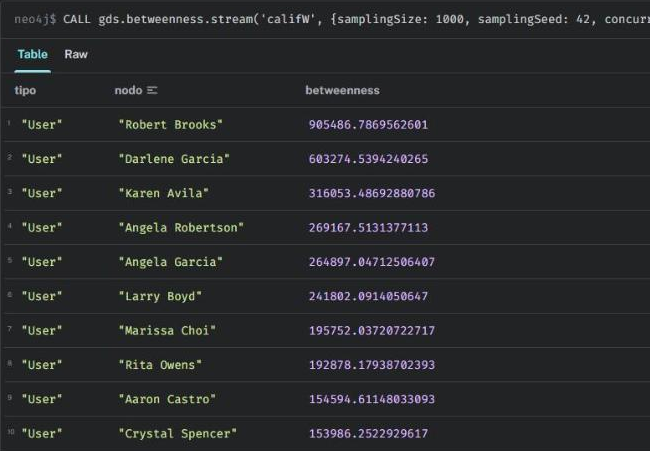
\includegraphics[width=7.1cm,height=\textheight]{img01.png}
\caption{1.5 --- modo stream}
\end{figure}

\begin{figure}
\centering
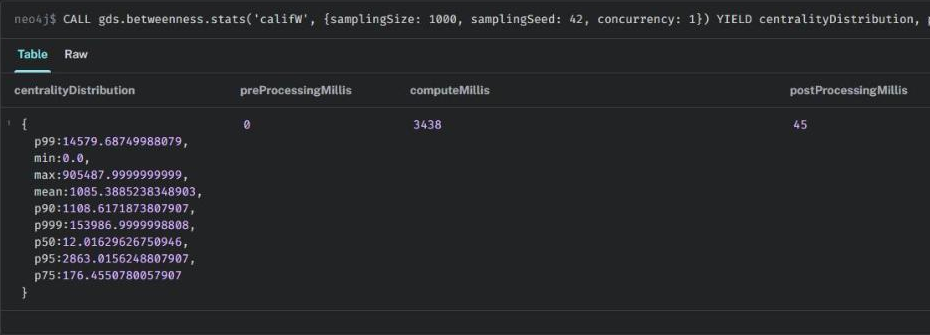
\includegraphics[width=10.2cm,height=\textheight]{img02.png}
\caption{1.5 --- modo stats}
\end{figure}

\begin{figure}
\centering
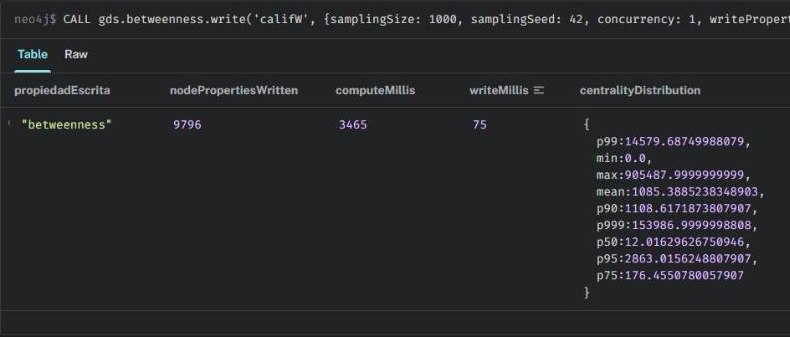
\includegraphics[width=8.7cm,height=\textheight]{img03.png}
\caption{1.5 --- modo write}
\end{figure}

\hypertarget{ejercicio-2-uxedndices-planes-y-escritura-por-lotes}{%
\subsection{Ejercicio 2 --- Índices, planes y escritura por
lotes}\label{ejercicio-2-uxedndices-planes-y-escritura-por-lotes}}

La consulta es
\texttt{MATCH\ (m:Movie)\ WHERE\ m.year\ \textgreater{}=\ 1990\ AND\ m.year\ \textless{}=\ 1999\ RETURN\ count(m)},
que devuelve 2.202 películas. \textbf{El dump ya trae un índice RANGE
sobre \texttt{Movie(year)}} (\texttt{index\_fc5f831e}). Para medir ``sin
el índice específico'', el script primero lo borra y controla que no
quede ninguno sobre \texttt{year}. Los tiempos del texto son la mediana
de 20 corridas después de un calentamiento. Cada captura muestra una
corrida suelta en Query, así que sus tiempos pueden diferir un poco; los
db hits y los operadores son los mismos.

\textbf{2.1 Sin índice.} El operador inicial es \textbf{NodeByLabelScan}
(recorre las 9.125 \texttt{:Movie}), seguido de \texttt{Filter}:
\textbf{18.222 db hits}, 9,0 ms de punta a punta y 6,89 ms de
operadores.

\begin{figure}
\centering
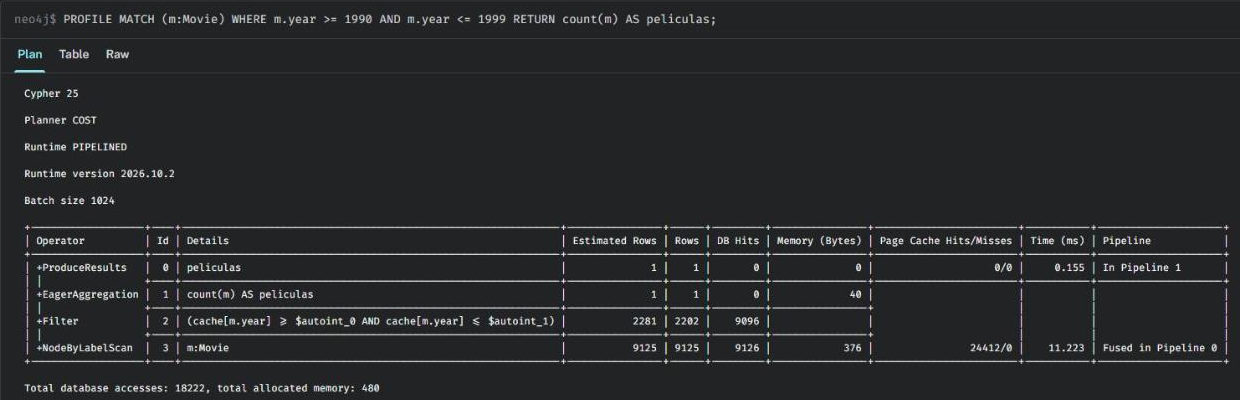
\includegraphics[width=13.6cm,height=\textheight]{img04.png}
\caption{2.1 --- PROFILE sin índice}
\end{figure}

\textbf{2.2 Con índice de rango \texttt{movie\_year\_range}.} El plan
pasa a \textbf{NodeIndexSeekByRange}, que lee solo las entradas del
rango: \textbf{2.203 db hits}, 2,0 ms de punta a punta y 0,73 ms de
operadores.

\begin{figure}
\centering
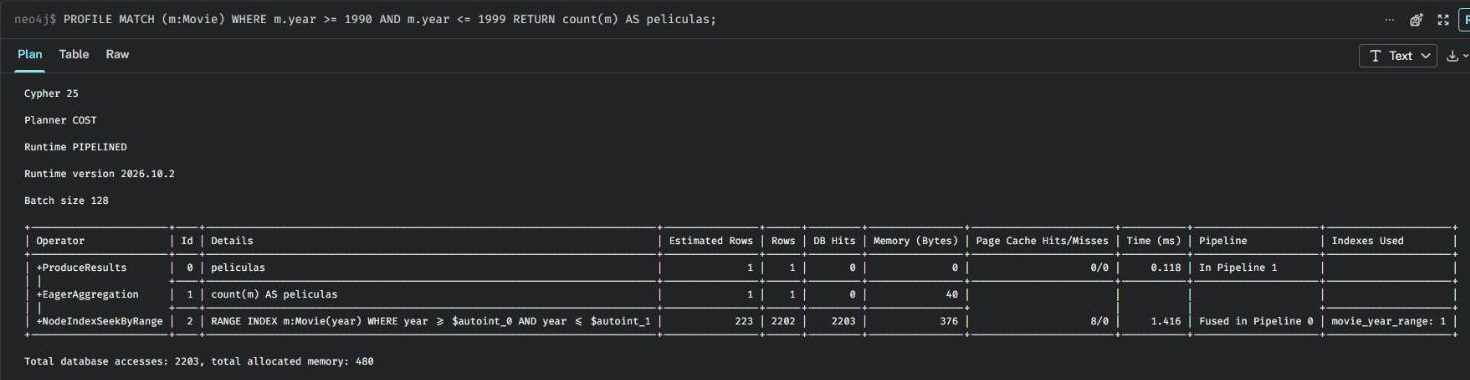
\includegraphics[width=16.2cm,height=\textheight]{img05.png}
\caption{2.2 --- PROFILE con índice de rango}
\end{figure}

\begin{longtable}[]{@{}ll@{}}
\toprule()
Factor de mejora (sin índice / con índice) & Valor \\
\midrule()
\endhead
db hits & \textbf{8,3×} \\
Tiempo de operadores (PROFILE) & \textbf{9,4×} \\
Tiempo de punta a punta (cliente) & 4,5× \\
\bottomrule()
\end{longtable}

La mejora en el motor (db hits y tiempo de operadores) es de casi un
orden de magnitud. De punta a punta es menor porque, con solo 9.125
películas, pesa el costo fijo del ida y vuelta con el servidor.

\textbf{2.3 EXPLAIN, runtime y Eager.} \texttt{EXPLAIN} muestra el plan
estimado sin ejecutar (sin filas ni db hits reales). \texttt{PROFILE}
confirma el \textbf{runtime PIPELINED} (planner COST, Cypher 25). En la
consulta de rango \textbf{no aparece Eager}, como se esperaba en una
lectura pura. Se analizó también la sentencia de escritura del 2.4: su
plan (\texttt{TransactionForeach} → \texttt{Expand} →
\texttt{EagerAggregation} → \texttt{Unwind} → \texttt{SetProperty})
\textbf{tampoco tiene un operador Eager}, porque lee \texttt{rating} y
escribe otra propiedad, \texttt{ratingNorm}, así que no hay conflicto de
lectura y escritura. \texttt{EagerAggregation} es la agregación que
calcula el promedio, no la barrera Eager.

\begin{figure}
\centering
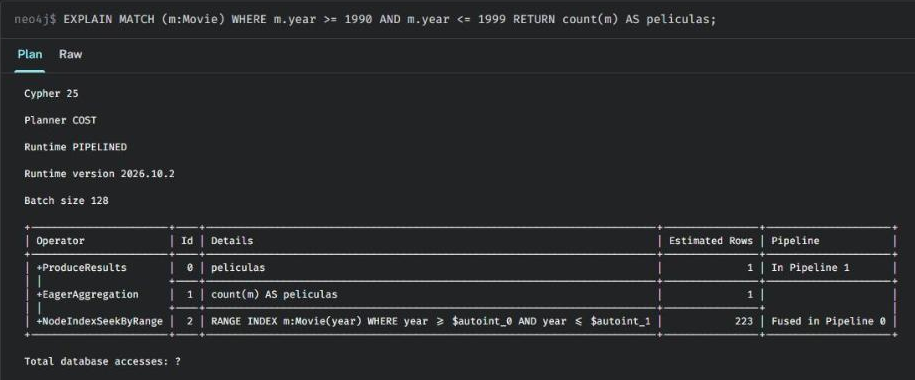
\includegraphics[width=10.1cm,height=\textheight]{img06.png}
\caption{2.3 --- EXPLAIN de la consulta de rango}
\end{figure}

\begin{figure}
\centering
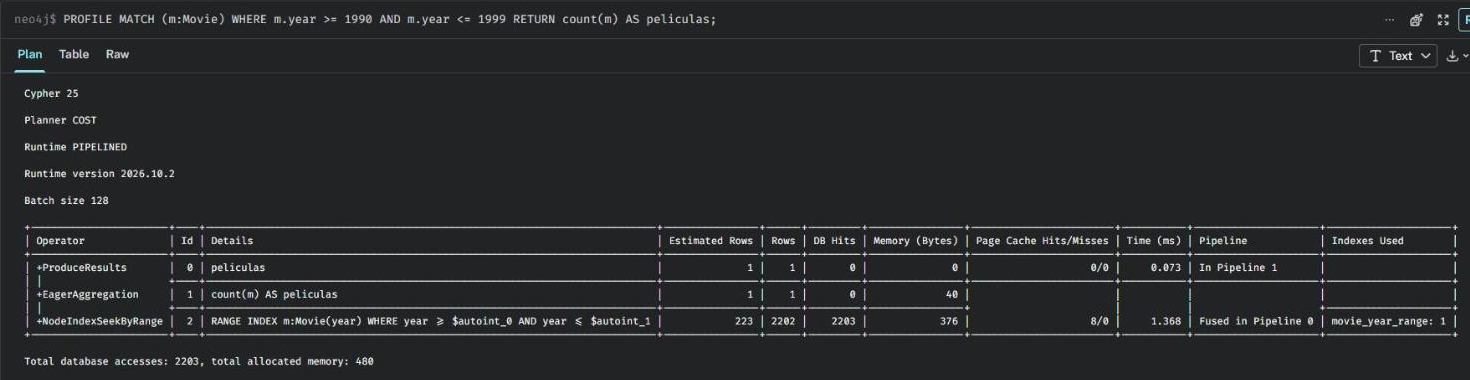
\includegraphics[width=16.2cm,height=\textheight]{img07.png}
\caption{2.3 --- PROFILE de la consulta de rango (runtime)}
\end{figure}

\begin{figure}
\centering
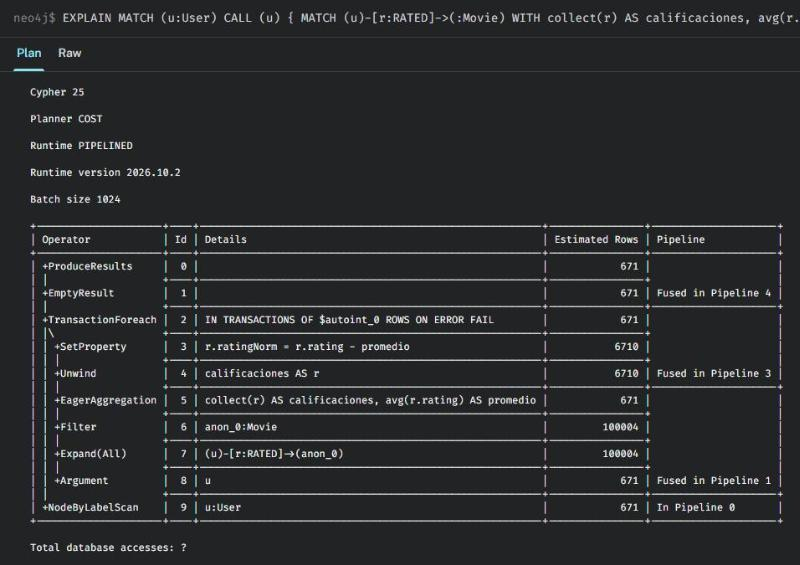
\includegraphics[width=8.8cm,height=\textheight]{img08.png}
\caption{2.3 --- EXPLAIN de la escritura del 2.4}
\end{figure}

\textbf{2.4 Escritura por lotes: \texttt{ratingNorm}.} Cada lote procesa
50 usuarios con todas sus calificaciones. El promedio del usuario se
calcula dentro de la transacción del lote:

\begin{verbatim}
MATCH (u:User)
CALL (u) {
  MATCH (u)-[r:RATED]->(:Movie)
  WITH collect(r) AS calificaciones, avg(r.rating) AS promedio
  UNWIND calificaciones AS r
  SET r.ratingNorm = r.rating - promedio
} IN TRANSACTIONS OF 50 ROWS;
\end{verbatim}

Verificación: todas las \texttt{{[}:RATED{]}} quedaron normalizadas y el
promedio de \texttt{ratingNorm} es 0, tanto global como por usuario.

\begin{longtable}[]{@{}lllll@{}}
\toprule()
RATED & Con ratingNorm & Promedio global & Mínimo & Máximo \\
\midrule()
\endhead
100.004 & 100.004 & 0,000 & -4,031 & 3,541 \\
\bottomrule()
\end{longtable}

\begin{longtable}[]{@{}llll@{}}
\toprule()
Usuario & Calificaciones & Promedio rating & Promedio ratingNorm \\
\midrule()
\endhead
Darlene Garcia & 2.391 & 3,367 & 0,000 \\
Robert Brooks & 1.868 & 3,552 & 0,000 \\
Karen Avila & 1.735 & 2,894 & 0,000 \\
Angela Garcia & 1.700 & 2,622 & 0,000 \\
Angela Robertson & 1.610 & 3,374 & 0,000 \\
\bottomrule()
\end{longtable}

\hypertarget{ejercicio-3-embeddings-predicciuxf3n-de-enlaces-y-pairre}{%
\subsection{Ejercicio 3 --- Embeddings, predicción de enlaces y
PairRE}\label{ejercicio-3-embeddings-predicciuxf3n-de-enlaces-y-pairre}}

\textbf{3.1 node2vec sobre \texttt{califW}.} Configuración: dimensión
128, \texttt{walkLength} 40, \texttt{walksPerNode} 10, una iteración,
caminatas sesgadas por el peso \texttt{rating}, semilla 42 y
\texttt{concurrency} 1. Se muestran 5 nodos (la ancla, la película más
calificada que no es la ancla y los 3 usuarios más activos), con las
primeras 6 de sus \textbf{128 componentes}. Los vectores completos están
en el Anexo:

\begin{longtable}[]{@{}
  >{\raggedright\arraybackslash}p{(\columnwidth - 6\tabcolsep) * \real{0.2500}}
  >{\raggedright\arraybackslash}p{(\columnwidth - 6\tabcolsep) * \real{0.2500}}
  >{\raggedright\arraybackslash}p{(\columnwidth - 6\tabcolsep) * \real{0.2500}}
  >{\raggedright\arraybackslash}p{(\columnwidth - 6\tabcolsep) * \real{0.2500}}@{}}
\toprule()
\begin{minipage}[b]{\linewidth}\raggedright
Tipo
\end{minipage} & \begin{minipage}[b]{\linewidth}\raggedright
Nodo
\end{minipage} & \begin{minipage}[b]{\linewidth}\raggedright
Dim.
\end{minipage} & \begin{minipage}[b]{\linewidth}\raggedright
Embedding (primeras 6 componentes)
\end{minipage} \\
\midrule()
\endhead
Movie & Forrest Gump & 128 & {[}0,146, -0,133, 0,241, 0,064, -0,284,
0,047, \ldots{]} (dim 128) \\
Movie & Pulp Fiction & 128 & {[}0,271, -0,089, 0,197, 0,052, -0,096,
-0,022, \ldots{]} (dim 128) \\
User & Darlene Garcia & 128 & {[}-0,796, -0,088, 0,122, -0,281, 0,279,
0,095, \ldots{]} (dim 128) \\
User & Karen Avila & 128 & {[}-0,610, -0,194, 0,113, 0,071, -0,130,
0,112, \ldots{]} (dim 128) \\
User & Robert Brooks & 128 & {[}0,109, -0,104, 0,078, 0,055, -0,048,
0,368, \ldots{]} (dim 128) \\
\bottomrule()
\end{longtable}

\textbf{3.2 Objetivo y subgrafo de entrenamiento.} Se predicen nuevas
\texttt{{[}:RATED{]}} usuario→película. El subgrafo se acotó, según las
NOTAS, a las películas con al menos 20 calificaciones (proyección Cypher
\texttt{califLP}): \textbf{1.974 nodos} (671 usuarios y 1.303 películas)
y \textbf{69.104 relaciones \texttt{{[}:RATED{]}}}. GDS informa 138.208,
porque cada arista no dirigida cuenta dos veces. Dentro del pipeline, el
split del 3.3 reparte esas relaciones así: ≈10 \% para test (≈6.910),
≈10 \% del resto como ejemplos positivos de entrenamiento del
clasificador (≈6.220) y el resto (≈55.970) como grafo de features, sobre
el que se calcula node2vec.

\textbf{3.3 Pipeline de link prediction.} node2vec es un \textbf{paso
del pipeline} (\texttt{addNodeProperty}): GDS lo recalcula sobre el
grafo de entrenamiento, así que las aristas de test no se filtran al
embedding. La feature es el producto de Hadamard de los embeddings.
Split: 10 \% test, 10 \% train del resto y 3 folds de validación, con
muestreo negativo 1:1. Candidatos: regresión logística (\texttt{penalty}
0, 0,01 y 0,1) y Random Forest (10 árboles con profundidad 10, y 25 con
profundidad 15). Métrica: AUCPR.

\begin{longtable}[]{@{}
  >{\raggedright\arraybackslash}p{(\columnwidth - 2\tabcolsep) * \real{0.5000}}
  >{\raggedright\arraybackslash}p{(\columnwidth - 2\tabcolsep) * \real{0.5000}}@{}}
\toprule()
\begin{minipage}[b]{\linewidth}\raggedright
Modelo candidato
\end{minipage} & \begin{minipage}[b]{\linewidth}\raggedright
AUCPR validación (media de 3 folds)
\end{minipage} \\
\midrule()
\endhead
Regresión logística, \texttt{penalty} 0 / 0,01 / 0,1 & 0,677 / 0,677 /
0,677 \\
Random Forest, 10 árboles y profundidad 10 & 0,815 \\
\textbf{Random Forest, 25 árboles y profundidad 15 (ganador)} &
\textbf{0,834} \\
\bottomrule()
\end{longtable}

\textbf{AUCPR de test = 0,832} (en \emph{outer-train}: 0,967). Con un
negativo por cada positivo, un clasificador al azar daría ≈0,5. La
regresión logística no logra separar bien el producto de Hadamard
(≈0,68); el bosque captura interacciones entre componentes y gana con
margen, aunque la brecha entre train y test muestra algo de sobreajuste.
El Random Forest devuelve la fracción de árboles que votan ``sí'':
\textbf{34 pares nuevos} (de 27 usuarios) empatan con probabilidad ≥
0,999. El top 5, obtenido con \texttt{concurrency} 1 para que sea
reproducible, es una selección entre esos empatados. Ninguno de los
pares existe en la base:

\begin{longtable}[]{@{}lllll@{}}
\toprule()
Usuario & Película & Año & Probabilidad & ¿Ya existe? \\
\midrule()
\endhead
Frank Davis & Jungle Book, The & 1967 & 1,0000 & no \\
Matthew Dudley & Parent Trap, The & 1961 & 1,0000 & no \\
Mrs.~Lisa Bradshaw & Hurricane, The & 1999 & 1,0000 & no \\
Mrs.~Lisa Bradshaw & Jacob's Ladder & 1990 & 1,0000 & no \\
Valerie Jackson & My Fair Lady & 1964 & 1,0000 & no \\
\bottomrule()
\end{longtable}

\textbf{3.4 Completado de KG con PairRE} (notebook
\texttt{ej3\_4\_pairre.ipynb}). Se usaron las tripletas
\texttt{IN\_GENRE} y \texttt{ACTED\_IN} de las películas con al menos 20
calificaciones: 8.719 tripletas y 4.052 entidades, con split 80/10/10 y
semilla 42. PairRE se entrenó con dimensión 128 y 100 épocas, en CPU. En
test filtrado: \textbf{MRR = 0,105} y \textbf{Hits@10 = 0,192}. Hechos
propuestos, \texttt{(película,\ IN\_GENRE,\ Drama)}, entre películas que
hoy no son Drama:

\begin{longtable}[]{@{}
  >{\raggedright\arraybackslash}p{(\columnwidth - 6\tabcolsep) * \real{0.2500}}
  >{\raggedright\arraybackslash}p{(\columnwidth - 6\tabcolsep) * \real{0.2500}}
  >{\raggedright\arraybackslash}p{(\columnwidth - 6\tabcolsep) * \real{0.2500}}
  >{\raggedright\arraybackslash}p{(\columnwidth - 6\tabcolsep) * \real{0.2500}}@{}}
\toprule()
\begin{minipage}[b]{\linewidth}\raggedright
Película
\end{minipage} & \begin{minipage}[b]{\linewidth}\raggedright
Género propuesto
\end{minipage} & \begin{minipage}[b]{\linewidth}\raggedright
Score
\end{minipage} & \begin{minipage}[b]{\linewidth}\raggedright
Géneros actuales
\end{minipage} \\
\midrule()
\endhead
Vanilla Sky (2001) & Drama & -2,569 & Mystery, Romance, Sci-Fi,
Thriller \\
African Queen, The (1951) & Drama & -2,592 & Adventure, Comedy, Romance,
War \\
Devil in a Blue Dress (1995) & Drama & -2,609 & Crime, Film-Noir,
Mystery, Thriller \\
\bottomrule()
\end{longtable}

Un ranking al azar daría Hits@10 ≈ 10/4.052 ≈ 0,0025, así que el modelo
es unas 75 veces mejor. Igual, el valor queda lejos del dataset
\emph{Nations} de la práctica (MRR ≈ 0,73) porque este KG es
\textbf{ralo}: unas 2,2 tripletas por entidad, y la mayoría de los
actores aparece una o dos veces. La pérdida converge hacia la época 20.
Los tres hechos propuestos son plausibles: \emph{Vanilla Sky} suele
describirse como drama psicológico, \emph{The African Queen} como
aventura romántica con mucho de drama, y \emph{Devil in a Blue Dress}
como drama criminal neo-noir. Se verificó contra Neo4j que hoy ninguna
de las tres tiene el género Drama. El score de PairRE es una distancia
con signo negativo: más alto es más plausible.

\hypertarget{anexo-vectores-node2vec-completos-punto-3.1}{%
\subsection{Anexo --- Vectores node2vec completos (punto
3.1)}\label{anexo-vectores-node2vec-completos-punto-3.1}}

Los 5 vectores de dimensión 128 del punto 3.1, con 2 decimales. Salen
del paso \texttt{3.1\_node2vec\_5\_nodos} de
\texttt{03\_ejercicio3.cypher} (semilla 42, \texttt{concurrency} 1,
reproducibles).

\begin{footnotesize}\sloppy
\noindent\textbf{Forrest Gump (Movie)}, dim 128: 0,15 -0,13 0,24 0,06 -0,28 0,05 0,00 0,57 -0,20 0,26 -0,23 -0,43 0,55 -0,28 0,04 -0,12 -0,10 0,37 -0,15 -0,06 0,25 0,09 0,02 0,19 -0,30 -0,04 -0,11 -0,23 -0,15 -0,09 -0,13 -0,11 0,31 -0,18 -0,26 -0,00 0,03 -0,16 0,22 -0,02 0,44 -0,45 0,09 -0,22 0,12 -0,22 -0,25 0,10 0,49 0,30 0,32 -0,29 0,29 0,48 0,14 -0,07 -0,04 0,13 0,09 -0,02 -0,36 0,24 0,23 -0,26 -0,22 -0,29 0,38 0,27 -0,30 0,23 -0,12 -0,10 -0,01 0,03 -0,46 0,04 0,20 -0,02 -0,06 0,02 0,05 0,01 -0,14 -0,20 -0,00 0,12 -0,09 0,44 0,41 -0,18 -0,21 -0,22 0,11 0,49 -0,18 0,03 -0,25 -0,12 0,21 -0,25 0,17 0,19 0,21 0,29 0,23 -0,15 -0,12 -0,16 -0,22 0,07 0,53 -0,12 0,10 -0,32 -0,20 -0,01 -0,06 -0,00 -0,34 0,12 -0,29 0,39 -0,58 -0,05 -0,04 0,09 0,23 -0,35\par\smallskip
\noindent\textbf{Pulp Fiction (Movie)}, dim 128: 0,27 -0,09 0,20 0,05 -0,10 -0,02 -0,09 0,27 -0,13 0,01 -0,17 -0,01 0,35 -0,02 -0,23 -0,14 0,18 0,19 -0,27 -0,15 -0,03 -0,25 0,15 0,16 -0,24 -0,05 -0,23 0,07 -0,35 -0,41 -0,27 -0,56 0,17 -0,00 -0,25 0,26 -0,05 0,13 -0,18 -0,15 0,02 -0,29 -0,06 -0,17 0,36 -0,18 -0,22 -0,07 0,43 0,23 0,28 -0,23 0,36 0,28 -0,02 -0,08 0,19 0,51 0,10 -0,00 -0,13 0,13 -0,04 -0,23 -0,14 -0,31 0,03 0,13 -0,52 -0,04 0,07 -0,19 -0,01 -0,10 -0,15 -0,13 0,25 0,15 -0,15 0,07 -0,20 -0,48 0,03 0,12 0,01 0,15 0,09 0,46 -0,08 -0,04 -0,05 0,15 -0,16 0,55 0,12 -0,29 -0,34 0,12 0,21 -0,33 -0,09 -0,02 0,39 0,41 0,27 -0,21 -0,05 -0,24 -0,24 -0,13 0,33 -0,05 0,44 0,19 -0,59 0,23 -0,15 -0,00 -0,21 -0,23 -0,27 0,12 -0,22 -0,07 -0,05 -0,04 0,39 0,05\par\smallskip
\noindent\textbf{Darlene Garcia (User)}, dim 128: -0,80 -0,09 0,12 -0,28 0,28 0,09 -0,50 -0,07 0,09 0,52 0,00 0,61 0,32 0,27 0,12 -0,17 0,04 0,12 -0,29 -0,13 0,34 0,14 0,29 0,26 -0,24 0,33 -0,10 0,38 -0,67 -0,33 -0,21 0,32 0,19 0,21 0,30 -0,16 0,14 0,59 0,36 0,40 -0,07 -0,22 -0,29 -0,07 -0,12 -0,08 -0,24 -0,17 0,79 -0,07 0,21 0,12 0,19 0,05 -0,14 0,05 -0,30 0,23 -0,12 -0,33 -0,06 0,10 -0,21 -0,19 0,02 -0,28 -0,24 -0,07 0,26 -0,24 0,06 0,08 -0,10 0,19 -0,18 0,28 0,22 0,05 0,22 0,45 0,04 -0,04 0,10 -0,10 0,34 0,33 -0,15 0,30 -0,45 -0,24 -0,16 -0,25 -0,57 0,26 0,04 0,11 -0,06 -0,11 0,20 -0,39 0,10 0,48 -0,15 0,14 -0,11 0,02 -0,13 -0,55 0,18 -0,15 0,36 0,52 0,10 0,06 0,21 0,29 -0,27 0,00 0,44 0,42 -0,24 0,08 -0,05 0,40 0,39 0,08 -0,37 -0,41\par\smallskip
\noindent\textbf{Karen Avila (User)}, dim 128: -0,61 -0,19 0,11 0,07 -0,13 0,11 0,14 0,19 0,17 -0,13 -0,26 0,15 0,41 -0,25 -0,12 0,02 0,34 -0,26 0,17 -0,18 -0,23 -0,05 -0,14 -0,31 -0,42 0,10 0,44 -0,09 -0,12 0,14 0,30 0,05 -0,02 -0,15 0,01 -0,12 0,35 0,16 0,14 -0,35 0,13 0,11 -0,16 0,33 0,04 0,13 0,05 0,36 1,00 0,60 0,12 -0,43 0,10 -0,18 0,54 0,52 0,12 -0,19 -0,10 -0,71 0,04 0,34 0,21 -0,13 0,44 -0,45 -0,09 -0,05 -0,89 -0,47 -0,16 -0,40 0,28 0,29 -0,04 0,31 0,36 -0,14 -0,12 0,14 -0,22 0,21 0,32 -0,12 0,24 0,34 -0,24 0,37 0,32 -0,17 -0,14 -0,23 -0,09 0,23 0,02 -0,43 -0,34 -0,06 -0,06 -0,69 -0,26 -0,22 0,47 0,17 0,20 0,30 0,10 0,01 -0,12 0,50 -0,37 0,19 -0,42 -0,42 -0,23 -0,30 -0,23 -0,16 -0,09 -0,38 -0,19 0,10 -0,25 0,04 -0,29 0,15 0,12 -0,15\par\smallskip
\noindent\textbf{Robert Brooks (User)}, dim 128: 0,11 -0,10 0,08 0,06 -0,05 0,37 0,08 0,11 0,26 0,41 0,02 -0,11 0,45 -0,30 -0,22 0,29 0,19 0,11 -0,01 -0,00 0,32 0,02 0,05 -0,04 0,11 0,20 -0,09 -0,17 -0,17 0,13 -0,03 0,02 -0,18 -0,22 -0,13 0,46 0,10 0,28 0,45 -0,17 0,45 -0,25 0,07 -0,06 -0,04 0,26 0,10 -0,16 0,76 0,04 0,08 -0,13 0,28 -0,25 -0,29 -0,15 0,09 -0,10 0,38 -0,07 0,01 0,14 0,42 -0,18 -0,20 -0,14 -0,10 0,21 -0,52 -0,12 -0,13 0,05 -0,16 0,64 0,05 -0,04 0,26 -0,17 -0,09 -0,22 -0,06 0,06 -0,32 0,16 0,07 0,26 -0,17 0,06 -0,29 -0,16 0,24 -0,35 0,22 0,40 0,11 -0,03 -0,51 0,05 0,24 -0,57 -0,08 -0,24 -0,09 -0,24 0,12 0,07 -0,04 0,14 -0,49 0,04 -0,03 0,33 0,27 0,13 -0,17 0,06 -0,17 0,18 -0,08 -0,29 0,62 -0,01 -0,18 -0,06 0,36 -0,14 0,08 -0,26\par\smallskip
\end{footnotesize}

\end{document}
